\documentclass{beamer}
%
% Choose how your presentation looks.
%
% For more themes, color themes and font themes, see:
% http://deic.uab.es/~iblanes/beamer_gallery/index_by_theme.html
%
\mode<presentation>
{
  \usetheme{Madrid}      % or try Darmstadt, Madrid, Warsaw, ...
  \usecolortheme{beaver} % or try albatross, beaver, crane, ...
  \usefonttheme{default}  % or try serif, structurebold, ...
  \setbeamertemplate{navigation symbols}{}
  \setbeamertemplate{caption}[numbered]
} 

\usepackage[english]{babel}
\usepackage[utf8x]{inputenc}

\title[Theory of languages]{Introduction to theory of languages}
\author{Patryk Kiepas}
\institute{MINES ParisTech \\ AGH University Of Science and Technology \\ THALES}

\date{\today}

\begin{document}

% --------------------------------------------------------------------- %
\begin{frame}
  \titlepage
\end{frame}

% Uncomment these lines for an automatically generated outline.
%\begin{frame}{Outline}
%  \tableofcontents
%\end{frame}

\section{Introduction}

% --------------------------------------------------------------------- %
\begin{frame}{Course plan}

\begin{enumerate}
\item Saturday, 25th of February 2017 -- lecture
\begin{itemize}
\item Languages
\item Grammars
\end{itemize}
\item Saturday, 4th of March 2017 -- lecture
\begin{itemize}
\item Parsing
\item ANTLR
\end{itemize}
\item Saturday, 11th of March 2017 -- exercises
\begin{itemize}
\item Grammars and languages
\item ANTLR
\end{itemize}
\item Saturday, 25th of March 2017 -- exercises \& exam (???)
\begin{itemize}
\item ANTLR
\end{itemize}
\end{enumerate}

\end{frame}

% --------------------------------------------------------------------- %
\begin{frame}[fragile]{Additional informations}
\begin{alertblock}{Any questions?}
Ask by mail: \verb|kiepas@agh.edu.pl|
\end{alertblock}

\begin{alertblock}{Course web-page}
\verb|http://home.agh.edu.pl/~kiepas| $\rightarrow$ \textbf{Teaching} $\rightarrow$ \textbf{Introduction to theory of languages (2017)}
\end{alertblock}
\end{frame}

% --------------------------------------------------------------------- %
\begin{frame}{This lecture}
\begin{itemize}
\item Linguistics
\item Languages
\item Grammar
\item Hierarchy of grammars
\item Notations
\item Automaton
\end{itemize}
\end{frame}

\section{Theory}

\subsection{Languages}

% --------------------------------------------------------------------- %
\begin{frame}{Introduction}

\begin{block}{Linguistics}
Scientific study of languages. Involves analysis of language:
\begin{itemize}
\item \textit{form} -- language evolution and task
\item \textit{context} -- environment of language usage
\item \textit{semantics} -- the meaning of the language
\end{itemize}
\end{block}

\begin{block}{Some important aspects}
\begin{itemize}
\item Phonetics
\item Articulation
\item Perception
\item Acoustic features
\item Morphology
\item Syntax
\end{itemize}
\end{block}

\end{frame}

% --------------------------------------------------------------------- %
\begin{frame}{Language types}
\begin{enumerate}
\item Natural languages
\begin{itemize}
\item \textit{Ordinary} -- evolves naturally in humans without planning
\item \textit{Controlled} -- a restricted subset of natural language in order reduce or eliminate ambiguity and complexity
\end{itemize}
\item \textbf{Artificial languages}
\begin{itemize}
\item \textit{Constructed} (planned \textit{a priori} or \textit{a posteriori})
\begin{itemize}
\item Engineered languages -- experiments in \textit{logic}, \textit{philosophy}, \textit{linguistics}
\item Auxiliary languages -- international communication (e.g. Esperanto, Ido,  Interlingua)
\item Artistic languages -- aesthetic pleasure or humorous effect (e.g. Klingon)
\end{itemize}
\item \textit{\textbf{Formal}}
\begin{itemize}
\item Computer programming languages (e.g. Java, Haskell, C, C++, Ruby)
\item Files and formats descriptions (e.g. YAML, JSON, XML)
\end{itemize}
\end{itemize}
\end{enumerate}
\end{frame}

% --------------------------------------------------------------------- %
\begin{frame}{Description of natural languages}

\begin{block}{A really small bit of history}
\begin{itemize}
\item In the late 1950's Noam Chomsky tried to describe natural languages
\item Important paper:  \textit{"Three models for the description of language"}, Noam Chomsky (1956).
\item In a result of his research two disciplines originated:
\begin{enumerate}
\item \textbf{\textit{Theory of formal grammars}}
\item \textit{Generative (transformational) grammars}
\end{enumerate}
\end{itemize}
\end{block}

\begin{figure}
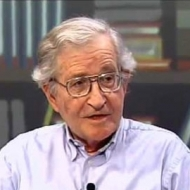
\includegraphics[width=0.2\textwidth]{img/noam_2.jpg}
\caption{\label{fig:your-figure}Professor of Linguistics (Emeritus) at MIT, Cambridge}
\end{figure}

\end{frame}

% --------------------------------------------------------------------- %
\begin{frame}{Description of natural languages}

\begin{block}{What we know now?}
\begin{itemize}
\item Description of natural languages is \textbf{hard}
\item Description of any natural languages might be \textbf{impossible}
\end{itemize}
\end{block}

\begin{block}{Why this is important?}
\begin{itemize}
\item Better understanding of language creation processes
\item More insights into functioning of our brain
\item \textbf{Natural language processing (NLP)}
\begin{itemize}
\item Translations (e.g. Google Translator)
\item Synthesis (e.g. speech generation)
\item Perceiving (e.g. robots, voice-control)
\end{itemize}
\end{itemize}
\end{block}

\end{frame}

% --------------------------------------------------------------------- %
\begin{frame}{Description of formal languages}

\begin{alertblock}{Result}
Description of natural languages help us describe an artificial (formal) ones
\end{alertblock}

\begin{block}{Programming languages}
\begin{itemize}
\item Protocol for communication with the computer
\item Performing operations and computations
\item Interpretation and execution
\item Compilation
\item Static code analysis
\end{itemize}
\end{block}

\begin{block}{Data formats}
\begin{itemize}
\item Structured data
\item Interchangeable model for communication and data transmission
\end{itemize}
\end{block}

\end{frame}

% --------------------------------------------------------------------- %
\begin{frame}{Alphabet}

\begin{block}{Alphabet}
A set $\Sigma$ of available symbols, the simplest elements in the language
\end{block}

\begin{exampleblock}{Examples}
\begin{itemize}
\item binary alphabet $\{0, 1\}$
\item decimal numbers $\{0,1,2,3,...,9\}$
\item Latin alphabet $\{a,b,c,d,...,z\}$
\item Cyrillic
\end{itemize}
\end{exampleblock}

\begin{figure}
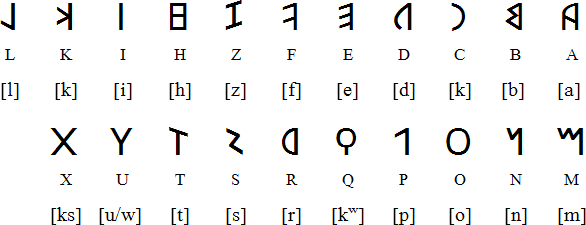
\includegraphics[width=0.5\textwidth]{img/latin_archaic.png}
\caption{\label{fig:latin_archaic}Ancient Latin alphabet}
\end{figure}

% --------------------------------------------------------------------- %
\end{frame}

\begin{frame}{Word (I)}
\begin{block}{Word}
Word $w$ is a sequence of $N$ symbols $w = x_1x_2...x_N$ (e.g. $010110$, $ABCDAAE$)
\end{block}

\begin{block}{Length}
Length of word $w$ is a number of symbols it consists of $|w|=N$ (e.g. $|010110| = 6$, $|ABCDAAE| = 7$)
\end{block}

\begin{alertblock}{Empty word}
Special word $\epsilon$ with length $|\epsilon|=0$
\end{alertblock}

\end{frame}

% --------------------------------------------------------------------- %
\begin{frame}{Word (II)}

\begin{exampleblock}{Words examples}
\begin{itemize}
\item $w = 010110$ word over alphabet $\Sigma = \{0, 1\}$
\item $w = abc13dj3$ word over alphabet $\Sigma = \{a, b, ...z, 0, 1, ...9\}$
\item $w = ACGTCCGGTA$ word over alphabet $\Sigma = \{A, C, G, T\}$
\end{itemize}
\end{exampleblock}

\begin{block}{Closures}
\begin{itemize}
\item $\Sigma^{\ast}$ -- set of all words over $\Sigma$
\item $\Sigma^{+}$ -- set of all nonempty words $\Sigma^+=\Sigma^*\backslash\{\epsilon\}$
\end{itemize}
\end{block}

\begin{exampleblock}{Closures examples}
\begin{itemize}
\item if $\Sigma = \{a\}$ then $\Sigma^{\ast} = \{\epsilon, a, aa, aaa, aaaa, aaaaa, aaaaaa, ...\}$
\item if $\Sigma = \{a, b\}$ then $\Sigma^{+} = \{a, b, aa, bb, ab, ba, aaa, bbb, ...\}$
\item if $\Sigma = \{a, b, ..., z\}$ then $\Sigma^{+} = \{cat, dog, a, aa, aaa, ...\}$
\end{itemize}
\end{exampleblock}

\end{frame}

% --------------------------------------------------------------------- %
\begin{frame}{Language}
	
\begin{definition}{Formal language}
$L$ is a set of words over an alphabet $\Sigma$, $L \subseteq \Sigma^{\ast}$
\end{definition}
	
\begin{exampleblock}{Examples}
\begin{itemize}
\item Language $L_1$ of palindromes in English $L_1 = \{mum, hannah, madam,...\}$
\item Morse code with alphabet $\Sigma=\{\cdot,	 -\}$, $L_2=\{\cdot -, - \cdot \cdot\,...,--\cdot\cdot\}$
\item Empty language
\item English language
\item Language $L_3$ with the set of words with fixed-size of N 
\end{itemize}
\end{exampleblock}
\end{frame}

\subsection{Grammar}

% --------------------------------------------------------------------- %
\begin{frame}{Grammar}

\begin{block}{Grammar}
\begin{itemize}
\item Description of a language
\item A recipe for composing elements into sentence
\item Describes syntax of a language
\end{itemize}
\end{block}

\begin{definition}{Grammar}
is a system $G = (\Sigma, NT, P, S)$ where:
\begin{itemize}
\item $\Sigma$ -- alphabet (set of terminals)
\item $NT$ -- set of nonterminals
\item $P$ -- set of production rules
\item $S$ -- marked nonterminal as \textit{start symbol}
\end{itemize}
\end{definition}

\end{frame}

% --------------------------------------------------------------------- %
\begin{frame}{Grammar and languages}

\begin{block}{Grammar properties}
\begin{itemize}
\item $NT, P$ -- are finite and nonempty
\item $\Sigma$ -- usually nonempty (if empty we have an empty language)
\item $\Sigma, NT$ -- are disjoint
\item $P \subseteq (\Sigma \cup NT)^{+} \times (\Sigma \cup NT)^{\ast}$
\item $S \in NT$
\end{itemize}
\end{block}

\begin{block}{Grammar and languages}
\begin{itemize}
	\item Sentence generated by some $G$ is every $w\in \Sigma^{\ast}$ for each exists derivation from $S$
	\item Language $L(G)$ is generated by $G$ and consists of sentences derivate using grammar $G$
	\item Two grammars $G_1$ and $G_2$ are \textit{(weakly) equivalent} if $L(G_1) = L(G_2)$
\end{itemize}
\end{block}

 \end{frame}

% --------------------------------------------------------------------- %
\begin{frame}{Grammar example}
\begin{examples}{Digits separated by plus or minus signs}
\begin{eqnarray*}
\begin{aligned}
& list \rightarrow list + list \\
& list \rightarrow list - list \\
& list \rightarrow \ 0 \ | \ 1 \ | \ 2 \ | \ 3 \ | \ 4 \ | \ 5 \ | \ 6 \ | \ 7 \ | \ 8 \ | \ 9
\end{aligned}
\end{eqnarray*}
\end{examples}
\end{frame}

% ---------------------------------------------------------------------%
\begin{frame}{Chomsky's hierarchy}

\begin{block}{Hierarchy}
\begin{itemize}
\item Describe the grammar expressiveness
\item Describe the grammar hardness
\item Tells us what ``mechanical procedure`` we need to use in order to:
\begin{itemize}
\item Accept language
\item Generate language
\end{itemize}
\item $\alpha, \beta$ -- any sequence of terminals and nonterminals
\item $\gamma$ -- any nonempty sequence of terminals and nonterminals
\item $A, B$ -- nonterminals
\end{itemize}
\end{block}

\begin{table}\footnotesize
\begin{tabular}{c|c|c|c}
Grammar & Language & Automaton & Production rules \\
\hline
Type-0 & Recursively enumerable & Turing machine &  $\alpha \rightarrow \beta$ \\ %Turing machine 
Type-1 & Context-sensitive & Linear bounded ND TM &$\alpha A\beta \rightarrow \alpha \gamma \beta$ \\ 
Type-2 & Context-free & ND pushdown & $\alpha \rightarrow \gamma$ \\ 
Type-3 & Regular & Finite state &$A\rightarrow a$ and $A\rightarrow aB$ 
\end{tabular}
\end{table}

%\begin{figure}
%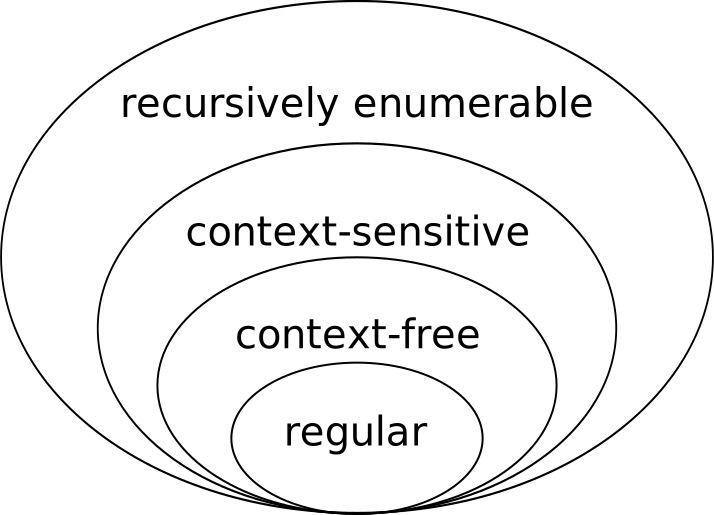
\includegraphics[width=0.2\textwidth]{img/Chomsky-hierarchy.svg}
%\caption{\label{fig:your-figure}Professor of Linguistics (Emeritus) at MIT, Cambridge}
%\end{figure}

\end{frame}

% --------------------------------------------------------------------- %
%\begin{frame}{Limiting condition}

%\begin{block}{First condition}
%Production rules can't decrease length of word. $\forall (\alpha \rightarrow \beta)\in P : |\alpha| \leq |\beta|$
%\end{block}

%\begin{block}{Second condition}

%\end{block}

%\begin{block}{Third condition}

%\end{block}

%\end{frame}

% --------------------------------------------------------------------- %
%\begin{frame}{Type-0: Unrestricted grammar}
%\end{frame}

% --------------------------------------------------------------------- %
%\begin{frame}{Type-1: Context-sensitive grammar}
%\end{frame}

% --------------------------------------------------------------------- %
%\begin{frame}{Type-2: Context-free grammar}
%\end{frame}

% --------------------------------------------------------------------- %
%\begin{frame}{Type-3: Regular grammar}
%\end{frame}

\subsection{Notation}

% --------------------------------------------------------------------- %
\begin{frame}[fragile]{Backus-Naur form (BNF)}

\begin{block}{Backus-Naur form (BNF)}
Notation technique for \textit{context-free grammars}. Frequently used to describe syntax of \textit{programming languages}, \textit{document formats} etc.
\end{block}


\begin{block}{Syntax}
\begin{verbatim}
                 <term> ::= __expression__
\end{verbatim}
\vskip -0.5cm
\begin{itemize}
\item \verb|<term>| is a \textit{nonterminal}
\item \verb|__expression__| is a sequence of one or more terminal and/or nonterminal symbols separated by vertical line \verb$|$
\item Terminal symbols: \verb|a|, \verb|b|, \verb|c|, \verb|A|, \verb|0|, \verb|1|, \verb|2| etc.
\item Nonterminal symbols: \verb|<digit>|, \verb|<postal-code>| etc.
\end{itemize}
\end{block}

\end{frame}

% --------------------------------------------------------------------- %
\begin{frame}[fragile]{Backus-Naur form (BNF)}

\begin{block}{Meta-symbols}
\begin{itemize}
\item $::=$ -- production rule definition
\item $|$ -- rule alternative
\item $< >$ -- nonterminals
\item $""$ -- literal
\item $<EOL>$ -- End Of Line
\end{itemize}
\end{block}

\begin{exampleblock}{Examples}
\small
\begin{verbatim}
<digit> ::= 0 | 1 | 2 | 3 | 4 | 5 | 6 | 7 | 8 | 9
<postal-code> ::= <digit> <digit> <digit> <digit> <digit>
\end{verbatim}
\end{exampleblock}

\end{frame}

% --------------------------------------------------------------------- %
\begin{frame}[fragile]{BNF example : Palindrome}

\begin{exampleblock}{Palindrome grammar}
\begin{verbatim}
<letter>     ::= a | b | c | ... | y | z
<palindrome> ::= <letter> |
<palindrome> ::= a <palindrome> a | b <palindrome> b |
                 c <palindrome> c | d <palindrome> d | 
                 e <palindrome> e | ...
                                  | z <palindrome> z
\end{verbatim}
\end{exampleblock}

\begin{exampleblock}{Results}
\begin{verbatim}
a
bb
bab
pop
hannah
\end{verbatim}
\end{exampleblock}

\end{frame}

% --------------------------------------------------------------------- %
\begin{frame}[fragile]{BNF example : Postal address}
\begin{exampleblock}{Postal address grammar}\small
\begin{verbatim}
<postal-address> ::= <name-part> <street-address> <zip-part>
<name-part> ::= <first-name> <last-name> <EOL> 
<street-address> ::= <number> <street-name> <apt-num> <EOL>
<zip-part> ::= <postal-code> <town-name> <EOL>
<apt-num> ::= <number> | ""
\end{verbatim}
\end{exampleblock}
\end{frame}

% --------------------------------------------------------------------- %
%\begin{frame}{Extended Backus-Naur form (EBNF)}
%\end{frame}

\section{Parsing}

\subsection{Methods}

\subsection{Tools}

% --------------------------------------------------------------------- %
%\begin{frame}{ANTLR}
%\end{frame}

% Commands to include a figure:
%\begin{figure}
%\includegraphics[width=\textwidth]{your-figure's-file-name}
%\caption{\label{fig:your-figure}Caption goes here.}
%\end{figure}


\end{document}
